\documentclass[12pt,a4paper,openright,twoside]{book}
\usepackage[utf8]{inputenc}
\usepackage{disi-thesis}
\usepackage{code-lstlistings}
\usepackage{notes}
\usepackage{shortcuts}
\usepackage{acronym}

\school{\unibo}
\programme{Corso di Laurea in Ingegneria e Scienze Informatiche}
\title{Integrazione di RAG e LLM nello Sviluppo del Software}
\author{Bollini Simone}
\date{\today}
\subject{Programmazione ad oggetti}
\supervisor{Prof. Viroli Mirko}
\cosupervisor{Dott. Aguzzi Gianluca}
\morecosupervisor{Dott. Farabegoli Nicolas}
\session{IV}
\academicyear{2023-2024}

% Definition of acronyms
\acrodef{RAG}{Retrieval-Augmented Generation}
\acrodef{AI}{Artificial intelligence}
\acrodef{LLM}{Large Language Model}


\mainlinespacing{1.241} % line spacing in mainmatter, comment to default (1)

\begin{document}

\frontmatter \frontispiece

\begin{abstract}	
I \ac{LLM} addestrati per sviluppare il codice sono oggi altamente efficaci e in grado di generare soluzioni utili e funzionanti.
L'addestramento fatto dai modelli è però su fonti e soluzioni generali, questo non da quindi la possibilità al modello di proppore soluzioni su misura per una specifica richiesta utilizzando casistiche già create dal programmatore o dalla propria azienda per casi simili. Da questo nasce l'esigenza di addestrare il modello per personalizzare le soluzioni proposte, contestualizzandole alla propria realtà aziendale e al proprio stile nel programmare.
Il \ac{LLM} non conosce le librerie interne dell'azienda, i pattern di programmazione adottati e quindi le risposte ottenute sono troppo generiche.
Per rispondere a questa esigenza entra in gioco la \ac{RAG} ovvero il processo di ottimizzazione dell'output di un \ac{LLM}, per permettergli di fruire una base di conoscenza personalizza, unica e privata, questa \textbf{matrice di conoscenza}  si inserisce tra quanto già appreso dal modello dai dataset utilizzati in fase di addestramento, estendendo la base dati sulla quale generare l'output con la risposta.
Questa tesi sperimenta l'integrazione di un \ac{RAG} con un \ac{LLM} per ottenere dal modello risposte personalizzate con conoscenze private e specifiche fornite da un dataset personalizzato.


\end{abstract}

\begin{dedication}
A Giulia e ai miei figli, il dono più grande.
\newline A tutta la mia famiglia.
\newline Grazie a tutti voi.
\end{dedication}

%----------------------------------------------------------------------------------------
\tableofcontents   
\listoffigures     % (optional) comment if empty
\lstlistoflistings % (optional) comment if empty
%----------------------------------------------------------------------------------------

\mainmatter

%----------------------------------------------------------------------------------------
\chapter{Introduzione}
\label{chap:introduction}
%----------------------------------------------------------------------------------------

\section{Essere programmatori nel 2025}
Sono disponibili tantissimi (IDE) per lo sviluppo del codice uno di questi è \textbf{Visual Studio Code}, mentre \textbf{Github} può essere lo strumento utilizzato per contenere e condividere progetti per lavore in maniera collaborativa. Può anche essere molto utile, \textbf{COLAB} che permette di eseguire in remoto codice che richiede molta memoria su GPU spesso non disponbili localmente.
Questi esempi mostrano una panoramica vasta e complessa, con un frequente cambio di software per realizzare un programma, modifiche fatte localmente su Visual Studio Code vengono trasferite su GitHub e poi riprese su Colab dove a sua volta vengono eseguiti Commit e Push sul progetto radice presente su GitHub.
La cosa che accomuna questi strumenti oggi è che dispongono tutti di assistenti di programmazione basati sull'intelligenza artificiale, in grado di completare il codice, suggerire correzioni e creare documentazione pertinente.
Lo schema di lavoro appenda descritto è stato da me attuato per realizzare questa tesi, ho utilizzato Visual Studio Code per scrivere il codice Pyhon, GitHub per condividere il progetto e Colab per eseguire la maggior parte del codice.
Una delle funzionalità offerte da questi assistenti è la la funzione di \textbf{Github Copilot} 'Generate Commit Message with Copilot' che propone il testo da utilizzare come descrizione di un commit, ho provato a riscontrare quanto fosse contestualizzato e coerente 
con quanto aggiornato e ho ottenuto il seguente risultato:
\begin{figure}[h]
    \centering
    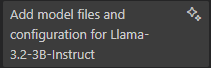
\includegraphics[width=0.5\linewidth]{figures/commit.png}
    \label{fig:Commeit-Autogenerato}
\end{figure}
\newline
Ho trovato coerente e giusto quanto proposto ed eseguito il Commit.
Quanto è riuscito a fare Copilot è strabiliante, in pochi istanti ha analizzato il contesto dando come output una risposta semplice ma coerente rispetto a quanto cambiato.
L'uso di questi strumenti rende il lavoro molto più dinamico e permette di ridurre le interruzioni per cercare una soluzione o per trovare le giuste parole per descrivere
quanto fatto.
\begin{figure}[h]
    \centering
    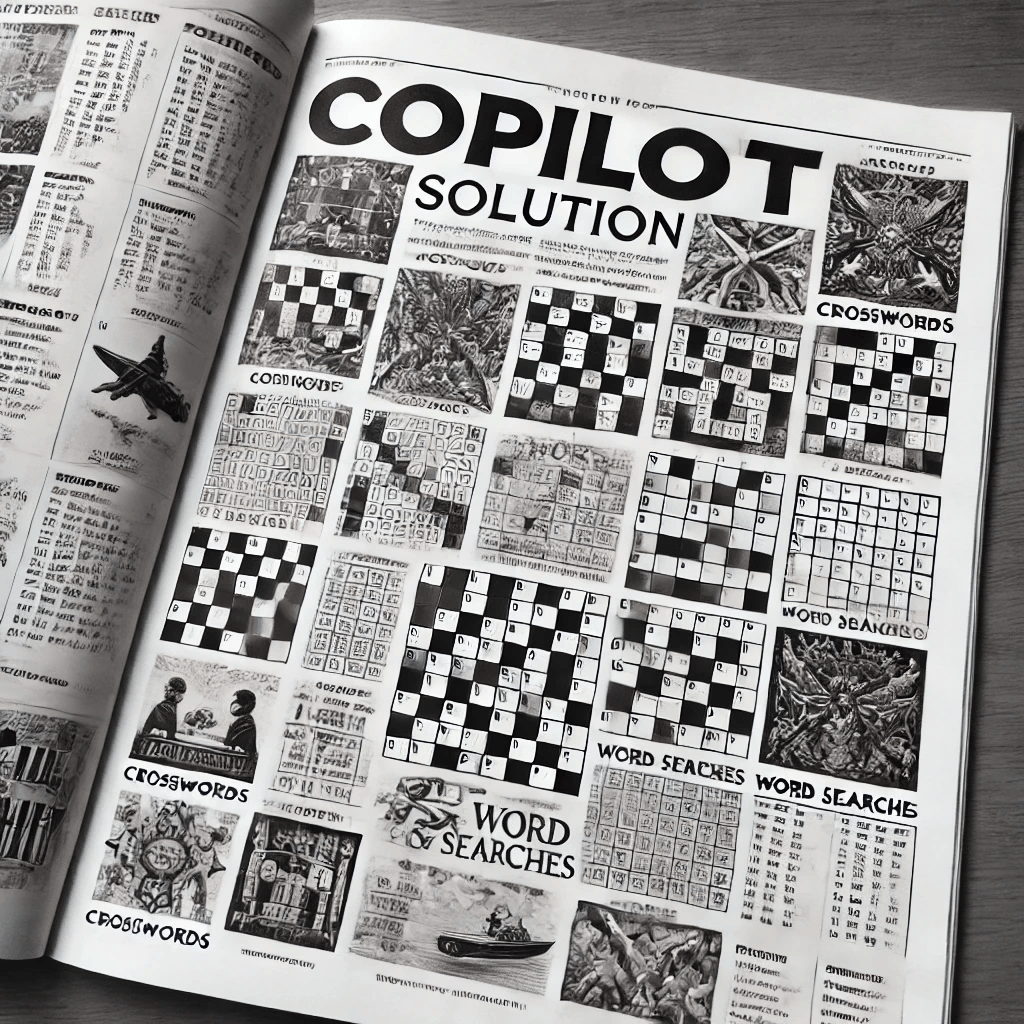
\includegraphics[width=0.5\linewidth]{figures/copilotsolutionSettimanaEnigmistica.png}
    \label{fig:Copilot-Solution}
\end{figure}
\newline
L'intelligenza artificiale sta rivoluzionando il modo in cui il software viene sviluppato, dando la possibilità a strumenti come Copilot di esplodere tutto il loro potenziale permettono di creare la spina dorsale di un progetto lasciando al programmatore il compito di verificare e correggere solo in parte il codice perché indirizzati e condizionati da quanto proposto. 
In progetti complessi questo non riduce il ruolo del programmatore, anzi lo eleva a compiti più precisi e complessi lasciando la stesura di parti del codice semplici e ripetitive al software stesso.
Sapere cosa chiedere e formulare correttamente le domande al LLM è fondamentale, esplicitando nel dettaglio con parole chiave mirate come deve essere realizzato il codice.
Altro compito complesso per il programmatore è non farsi troppo ammaliare dalle soluzioni proposte perché non sempre necessarie per quanto richiesto oppure diversa da quanto già conosciuto per realizzare una determinata funzione.
Questo nuovo modo di lavorare per mette di conoscere nuove soluzioni ma comporta test e tempo non sempre disponibile.
Il programmatore deve avere il controllo del progetto accettando generazione del codice automatica solo dove consapevole di quanto proposto e del suo impatto anche in casi di revisione e manutenzione futuri.
L'ultimo miglio da percorrere è la personalizzazione delle risposte del LLM, per ottenere risposte coerenti con quanto già realizzato e conosciuto, per fare questo entra in gioco la RAG.
\chapter{Addestrare un LLM per la Generazione del Codice}

L'addestramento di LLM per la generazione di codice di programmazione richiede una serie di passaggi metodici e risorse computazionali significative.
Conoscere questo processo è utile per la successiva integrazione con la RAG.
La procedura si divide nelle selle seguenti fasi:

\section{Raccolta e Preparazione dei Dati}

La qualità e la quantità dei dati per l'addestramento è di primaria importanza per prepare un modello alla generazione di codice in maniera efficace.
È quindi essenziale utilizzare per il training codice sorgente proveniente da molteplici fonti tra cui codice sorgente, file Readme, documentazione tecnica, commenti nel codice,
pagine Wiki, API e discussioni su forum specializzati in programmazione.
In rete è possibile trovare diverso materiale open source tra cui dataset già etichettati. Alcuni dataset hanno un valore altissimo, per tutelare il costo per produrli per certi dataset è previsto il diritto d'autore.
I dati si dividono in due tipologie:
\begin{itemize}
    \item \textbf{Dati Strutturati}: seguono un formato specifico e predefinito.
    \item \textbf{Dati non Strutturati}: non sono organizzati e sono quindi più difficili da interpretare dal modello. 
\end{itemize}
La raccolta di dati va visionata con cura, se non si conosce la provenienza del codice è possibile che contenga bug o codice opsoleto che possono essere trasmessi al modello.
I dati raccolti devono essere quindi puliti e pre-processati per rimuovere errori e informazioni non pertinenti, garantendo così un dataset di alta qualità per l'addestramento.
Sui dataset viene utilizzato un tokenizer specializzato che riconosce costrutti di programmazione come keyword, operatori e strutture sintattiche.

\section{Pre-Addestramento}
Il pre-addestramento di un LLM  da utilizzare per la generazione di codice richiede un approccio specifico.
A differenza del pre-addestramento generico, utilizzando i dataset precedentemente prepareti il modello impara a:
\begin{itemize}
    \item Predire il completamento del codice
    \item Comprendere la struttura sintattica dei linguaggi di programmazione
    \item Riconoscere pattern comuni nel codice
    \item Identificare le relazioni tra diversi blocchi di codice
\end{itemize}
Un esempio pratico di pre-addestramento può essere implementato utilizzando la libreria transformers \cite{huggingface-transformers, codebert}:

\begin{lstlisting}[language=Python]
from transformers import RobertaConfig, RobertaTokenizerFast

# Configurazione del modello per il codice
config = RobertaConfig(
    vocab_size=50000,  # Dimensione del vocabolario
    max_position_embeddings=514,  # Lunghezza massima sequenza
    num_attention_heads=12,  # Teste di attenzione
    num_hidden_layers=6,  # Strati nascosti
    type_vocab_size=1  # Tipo di vocabolario
)

# Tokenizer specializzato per il codice
tokenizer = RobertaTokenizerFast.from_pretrained(
    "microsoft/codebert-base",
    max_length=512,
    truncation=True,
    padding=True
)
\end{lstlisting}

Durante questa fase, il modello sviluppa una comprensione profonda della sintassi e della semantica del codice, che verrà poi raffinata durante il fine-tuning per compiti specifici di generazione del codice.
\section{Fine-Tuning}
Il fine-tuning è la fase in cui il modello viene specializzato per la generazione di codice, documentazione e risposta a quesiti specifici del contesto di programmazione. Durante questa fase, il modello affina le sue capacità attraverso:

\begin{itemize}
    \item \textbf{Dataset Specializzati}: Utilizzo di dataset contenenti:
    \begin{itemize}
        \item Coppie di descrizioni-implementazioni
        \item Documentazione tecnica e commenti
        \item Esempi di bug fixing e refactoring
    \end{itemize}
    
    \item \textbf{Tecniche di Apprendimento}:
    \begin{itemize}
        \item \textbf{Apprendimento Supervisionato}: Training su coppie input-output predefinite
        \item \textbf{Apprendimento per Rinforzo}: Ottimizzazione basata su feedback e metriche di qualità
        \item \textbf{Few-shot Learning}: Adattamento a nuovi contesti con pochi esempi
    \end{itemize}
\end{itemize}

Un esempio pratico di fine-tuning può essere implementato utilizzando la libreria transformers \cite{huggingface-transformers}:

\begin{lstlisting}[language=Python]
from transformers import Trainer, TrainingArguments
from datasets import load_dataset

# Caricamento del dataset per il fine-tuning
dataset = load_dataset("code_search_net", "python")

# Configurazione del training
training_args = TrainingArguments(
    output_dir="./results",
    num_train_epochs=3,
    per_device_train_batch_size=8,
    per_device_eval_batch_size=8,
    warmup_steps=500,
    weight_decay=0.01,
    logging_dir="./logs",
    logging_steps=10,
    evaluation_strategy="epoch"
)

# Inizializzazione del trainer
trainer = Trainer(
    model=model,                # Modello pre-addestrato
    args=training_args,         # Argomenti di training
    train_dataset=dataset["train"],
    eval_dataset=dataset["validation"],
    tokenizer=tokenizer,        # Tokenizer specializzato per il codice
)

# Avvio del fine-tuning
trainer.train()
\end{lstlisting}

Durante il fine-tuning, il modello sviluppa capacità specifiche come:
\begin{itemize}
    \item Generazione di codice a partire da descrizioni in linguaggio naturale
    \item Completamento intelligente del codice basato sul contesto
    \item Creazione di documentazione tecnica
    \item Identificazione e correzione di bug
    \item Refactoring del codice seguendo best practices
\end{itemize}

Il processo di fine-tuning richiede un attento bilanciamento tra:
\begin{itemize}
    \item \textbf{Overfitting}: Evitare che il modello memorizzi i dati di training
    \item \textbf{Generalizzazione}: Mantenere la capacità di adattarsi a nuovi contesti
    \item \textbf{Prestazioni}: Ottimizzare la velocità e la qualità delle risposte
\end{itemize}

\section{Pre-Addestramento vs Fine-Tuning}
È importante comprendere la distinzione tra queste due fasi dell'addestramento:
\textbf{Pre-Addestramento}\newline
Il pre-addestramento è la fase iniziale dove il modello:
\begin{itemize}
    \item Acquisisce una comprensione \textbf{generale} del linguaggio di programmazione
    \item Viene addestrato su \textbf{grandi quantità} di codice sorgente generico
    \item Impara le strutture base e la sintassi del linguaggio
    \item Non è ancora specializzato per compiti specifici
\end{itemize}

\textbf{Fine-Tuning}\newline
Il fine-tuning è invece la fase di specializzazione dove il modello:
\begin{itemize}
    \item Si adatta a un \textbf{dominio specifico} o a compiti particolari
    \item Utilizza dataset più piccoli ma \textbf{mirati}
    \item Affina le conoscenze per generare codice specifico per il tuo caso d'uso
    \item Viene ottimizzato per le esigenze specifiche del progetto
\end{itemize}

\textbf{Analogia}: Si può paragonare a:
\begin{itemize}
    \item Pre-addestramento: Imparare la grammatica e il vocabolario di base di una lingua
    \item Fine-tuning: Specializzarsi nel linguaggio tecnico di un settore specifico
\end{itemize}

\section{Architettura del Modello}
Gli LLM utilizzano tipicamente architetture basate su trasformatori, che sono particolarmente efficaci nell'elaborazione di sequenze di dati, come il testo e il codice. I trasformatori utilizzano meccanismi di auto-attenzione per valutare l'importanza di diversi elementi in una sequenza, permettendo al modello di comprendere le relazioni a lungo raggio tra parole o token. Questa capacità è cruciale per la generazione di codice, dove le dipendenze tra variabili e funzioni possono estendersi su intere porzioni di codice.

\section{Valutazione e Ottimizzazione}
Una volta addestrato, il modello deve essere rigorosamente valutato utilizzando metriche specifiche per la generazione di codice, come la correttezza sintattica, la funzionalità e l'efficienza del codice prodotto. I risultati della valutazione guidano ulteriori ottimizzazioni, che possono includere aggiustamenti dei pesi del modello, modifiche all'architettura o l'inclusione di dati di addestramento aggiuntivi per affrontare eventuali carenze.

\subsection{Metriche di Valutazione}
\begin{itemize}
    \item \textbf{Correttezza Sintattica}: Verifica che il codice generato sia sintatticamente corretto.
    \item \textbf{Funzionalità}: Verifica che il codice generato realizzi la funzionalità desiderata.
    \item \textbf{Efficienza}: Valuta le prestazioni del codice in termini di tempo di esecuzione e utilizzo delle risorse.
\end{itemize}

\subsection{Tecniche di Ottimizzazione}
\begin{itemize}
    \item \textbf{Aggiustamento dei Pesi}: Modifica dei pesi del modello per migliorare le prestazioni.
    \item \textbf{Modifiche all'Architettura}: Introduzione di nuove componenti o modifiche a quelle esistenti.
    \item \textbf{Integrazione di Dati Aggiuntivi}: Utilizzo di ulteriori dati di addestramento per migliorare le prestazioni.
\end{itemize}

\chapter{RAG}
\section{Introduzione}
Il RAG \textbf{Retrieval-Augmented Generation}, (in italiano \textit{Generazione Aumentata tramite Recupero} )  è un sistema che permette di migliorare l'output di un LLM estendendo la sua conoscenza con nuove informazioni, al di fuori dai suoi dati di addestramento.
Allo scopo di:
\begin{itemize}
    \item ottenere risposte personalizzate provenienti da librerie e codice custom;
    \item migliorare il codice generato rendendolo più specifico al dominio riducendo le allucinazioni;
    \item facilitare l'assistenza da parte del modello nella fase di debugging migliorando la sua comprensione di sistemi complessi;
    \item supportare la creazione di documentazione aggiornata;
    \item permettere all'interno di un Team di migliorare la coerenza del codice scritto da diversi programmatori;
    \item realizzare naturalmente senza forzature, codice più moderno proponendo librerie e standard comuni.
    \item evitare risposte imprecise a causa della confusione terminologica, in cui diverse fonti utilizzano la stessa terminologia per parlare di cose diverse.
\end{itemize}

\section{Funzionamento}

\begin{figure}[h]
    \centering
    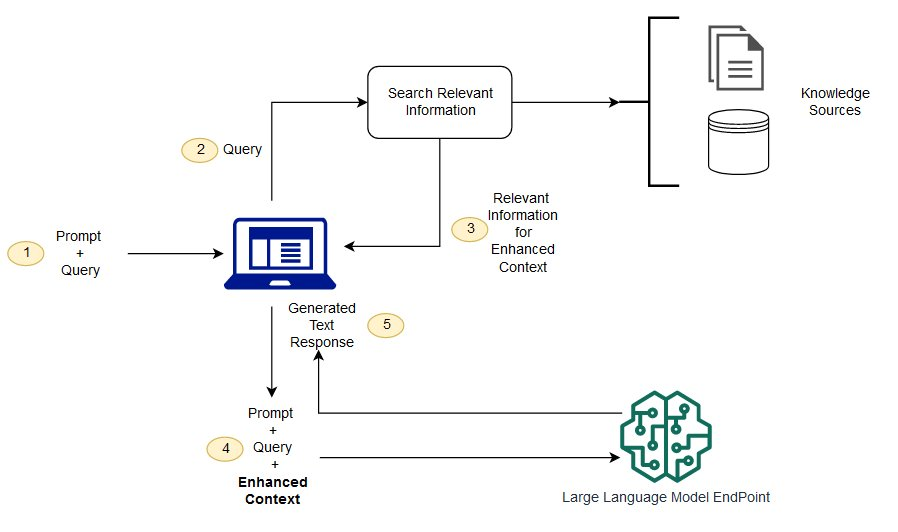
\includegraphics[width=.8\linewidth]{figures/jumpstart-fm-rag.jpg}
    \caption{Flusso di una request ad un LLM integrato con un RAG}
    \label{fig:jumpstart-fm-rag}
\end{figure}
RAG è un sistema che integra il processo di generazione del linguaggio con un meccanismo di recupero delle informazioni. Come illustrato in \cref{fig:jumpstart-fm-rag}, il funzionamento si articola in quattro fasi principali:

\subsection{Creazione di Dati Esterni}
Il sistema RAG utilizza dati esterni al training set originale del LLM, provenienti da diverse fonti come:
\begin{itemize}
    \item API e database
    \item Archivi documentali
    \item File di testo e codice
\end{itemize}
Questi dati vengono convertiti in rappresentazioni numeriche (embedding) e archiviati in un database vettoriale, creando una knowledge base accessibile al modello.

\subsection{Recupero delle Informazioni}
Quando l'utente sottopone una query:
\begin{itemize}
    \item La domanda viene convertita in un vettore
    \item Il sistema cerca nel database vettoriale le informazioni più pertinenti
    \item Viene calcolata la rilevanza attraverso calcoli matematici vettoriali
\end{itemize}

\subsection{Aumento del Prompt}
Il sistema RAG arricchisce il prompt dell'utente:
\begin{itemize}
    \item Aggiunge le informazioni recuperate al contesto
    \item Utilizza tecniche di prompt engineering per ottimizzare la comunicazione con il LLM
    \item Fornisce al modello un contesto arricchito per generare risposte più accurate
\end{itemize}

\subsection{Gestione dell'Aggiornamento}
Per mantenere l'efficacia del sistema nel tempo:
\begin{itemize}
    \item Aggiornamento asincrono dei documenti
    \item Ricalcolo degli embedding per i nuovi dati
    \item Possibilità di aggiornamenti in tempo reale o batch
\end{itemize}

Questo approccio permette di superare le limitazioni dei LLM tradizionali, fornendo risposte più accurate e contestualizzate grazie all'integrazione di conoscenze esterne aggiornate.

\chapter{Caso Studio: Implementazione di un Sistema RAG per lo Sviluppo del Software}

\section{Obiettivi del Caso Studio}
Questo caso studio si propone di:
\begin{itemize}
    \item Dimostrare l'applicazione pratica dei concetti teorici presentati nei capitoli precedenti
    \item \textbf{Scenario}: Supporto allo sviluppo software in una software-house
    \item \textbf{Problematica}: Necessità di generare codice coerente con gli standard e le pratiche aziendali
    \item \textbf{Soluzione Proposta}: Sistema RAG integrato con LLM per la generazione di codice contestualizzato
\end{itemize}


\section{Architettura del Sistema}
UML su lucidchart da completare
% \begin{figure}[h]
%     \centering
%     \includegraphics[width=.8\linewidth]{figures/rag-architecture.png}
%     \caption{Architettura del sistema RAG implementato}
%     \label{fig:rag-architecture}
% \end{figure}

\section{Software Utilizzati}
\subsection{Ollama}
Ollama \cite{ollama-docs} è un software che permette di utilizzare in locale LLM, facilitando la creazione, l'addestramento e l'integrazione di modelli di machine learning nelle applicazioni senza dover dipendere da servizi cloud esterni.
\subsection{LLM}
Per rendere più completa la ricerca sono stati utilizzati due modelli di linguaggio per il caso studio:
\subsubsection{Llama 3.2}
Llama 3.2 3B \cite{llama3-2}, un modello di linguaggio open source sviluppato da Meta AI.
Il modello, con 3 miliardi di parametri, è ottimizzato per compiti di dialogo multilingue e si distingue per le sue capacità di recupero e sintesi delle informazioni.
La scelta è ricaduta su questa versione per il suo equilibrio tra prestazioni e requisiti computazionali che permottono il suo utilizzo senza hardware troppo potente.

\subsubsection{qwen2.5-coder:3b}
qwen2.5-coder \cite{qwen-coder} è stato sviluppato da Qwen AI ed è anchesso open source, specializzato nella generazione di codice e documentazione tecnica.
Con 3 miliardi di parametri, il modello è stato addestrato su un ampio dataset di codice sorgente e documentazione tecnica, permettendo di generare codice coerente e ben strutturato. 
La scelta di questo modello è stata dettata, a differenza di llama3.2, dalla sua specializzazione nella programmazione e dalla sua capacità di generare codice di alta qualità.

\subsection{BGE-M3}
BGE-M3 \cite{bge-m3} è un database vettoriale open source per la gestione di dati strutturati e non strutturati multilingue, sviluppato da BigGraph Engine.
%\subsection{Google Colab}
%Utilizzate le schede video Tesla T4 di Google Colab per l'addestramento del modello.

\section{Dataset}
Il dataset utilizzato per il caso studio è stato creato a partire da documenti tecnici e codice sorgente di progetti interni all'azienda.

\section{Implementazione}
\subsection{Modello embedding}
Utilizzando BGE-M3 il contenuto del dataset viene suddivo in chunk e tramite il modello embeddig è convertito in rappresentazioni vettoriali numeriche.
esempio
\begin{lstlisting}[language=Python]
    model = BGEM3FlagModel('BAAI/bge-m3',  use_fp16=True)
    frase = "<cis-ui:button skin='red' text='Bottone rosso'/>"
    embeddings = model.encode(frase)['dense_vecs']
    print (embeddings)
\end{lstlisting}
\begin{verbatim}
    [-0.03712651  0.02731708 -0.03263818 ...  0.02965933 -0.01724784  0.00510089]
\end{verbatim}
l'output è un vettore numerico con 1024 elementi.


\chapter{Conclusioni}

\section{Risultati Ottenuti}
%In questa tesi ho esplorato l'integrazione di RAG e LLM nello sviluppo del software, dimostrando come questi strumenti possano migliorare significativamente il processo di sviluppo. I risultati principali includono:
%\begin{itemize}
%    \item Implementazione di un sistema RAG per la generazione di codice contestualizzato
 %   \item Analisi delle prestazioni e dell'efficacia del sistema
 %   \item Identificazione di potenziali aree di miglioramento
%\end{itemize}

\section{Impatto sullo Sviluppo Software}
L'integrazione di strumenti basati su AI nel processo di sviluppo software sta rivoluzionando il settore. Durante il periodo di sviluppo di questa tesi (Ottobre 2024 - Gennaio 2025), abbiamo osservato:
\begin{itemize}
    \item Rapida evoluzione degli strumenti di AI per lo sviluppo software
    \item Crescente disponibilità di soluzioni open source
    \item Miglioramento continuo nelle capacità di generazione e comprensione del codice
\end{itemize}

\section{Sfide e Prospettive Future}
%Nonostante i progressi significativi, rimangono diverse sfide da affrontare:
%\begin{itemize}
%    \item Bilanciamento tra automazione e controllo umano
%    \item Gestione delle implicazioni etiche
%    \item Necessità di mantenere competenze tecniche fondamentali
%\end{itemize}


%\lstinputlisting[float,language=Java,label={lst:random-code}]{listings/HelloWorld.java}


%----------------------------------------------------------------------------------------
% BIBLIOGRAPHY
%----------------------------------------------------------------------------------------

\backmatter

\nocite{*} % Remove this as soon as you have the first citation

\bibliographystyle{alpha}
\bibliography{bibliography}

\end{document}
